\section{The Large Hadron Collider}
\label{sec:LHC}

The Large Hadron Collider (LHC) \cite{LHCcern} is a 27km long particle accelerator about 100 meters below ground and is the most powerful of its kind in the world. Since the LHC replaced the other LEP-collider, the tunnel already existed which made the building a bit less comprehensive. The collider consists of superconducting magnets with accelerating structures to boost the proton velocity close to the speed of light, in an environment cooled down to 1.85K (-271.3$^o$C) to ensure superconductivity. The LHC accelerator is shown in figure \ref{fig:LHC} as part of a complex of CERN accelerators. 

\begin{figure}[H]
    \centering
    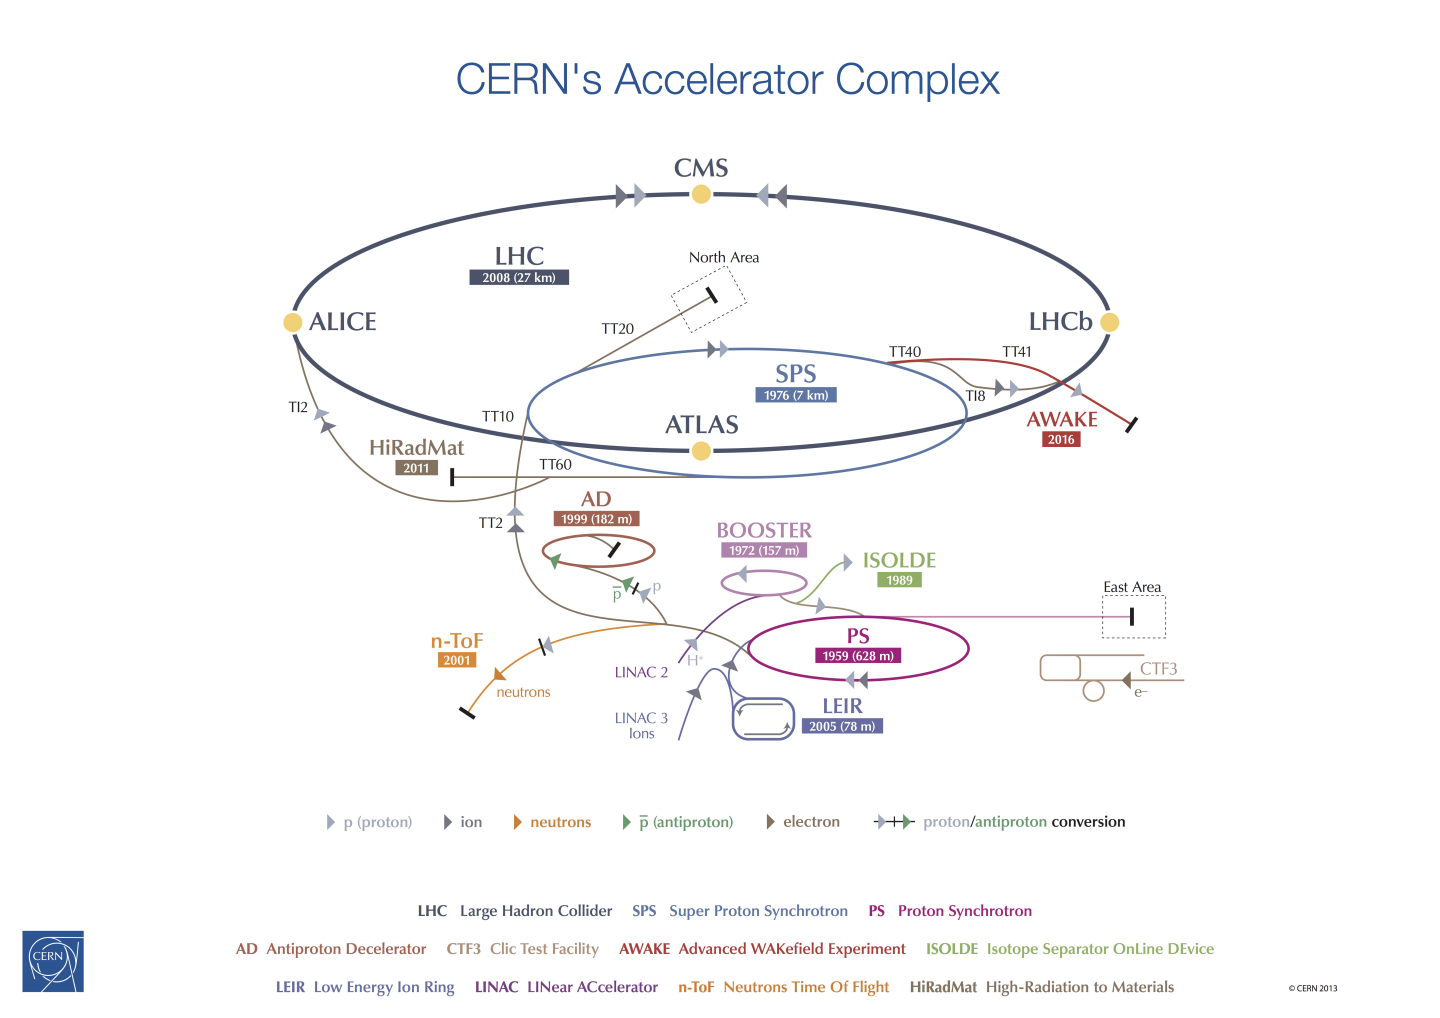
\includegraphics[width=\textwidth]{Figures/FromOnline/Poster-2013-377.jpg}
    \caption{An illustration of the accelerator complex at CERN \cite{LHCpic}}
    \label{fig:LHC}
\end{figure}

The protons extracted from a hydrogen bottle go through smaller accelerators to gain more energy before they, in the end, are injected in opposite directions into the LHC, which is the biggest circle in figure \ref{fig:LHC}. The particles get accelerated to about 99.99\% of the speed of light and a maximum energy of 6.5 TeV. In the end the two beams of protons collide in the centre of four experiments around LHC, which are marked with yellow dots in figure \ref{fig:LHC}, namely ATLAS, ALICE, CMS and LHCb. 

The different experiments focus on different research goals. ATLAS (A Toridal LHC ApparatuS) and CMS (Compact
Muon Solenoid) are multipurpose detectors mainly focusing on SM measurements and searches for new physics, i.e. discovery of new particles and phenomena, e.g. Supersymmetry and Dark Matter. The most famous achievement of ATLAS and CMS is the discovery of the Higgs boson. ALICE (A Large Ion Collider Experiment) focuses on heavy ion collisions with lead-lead and lead-proton to study the quark-gluon plasma. LHCb (Large Hadron Collider beaty) focuses on processes related to b-quarks to precisely measure CP violation and oscillation phenomena. 

At the LHC we focus on proton-proton collisions (and heavy ion collisions) to study various high energy final states via electroweak and strong interactions with the hope to discover new phenomena. The internal structure of the proton allows to register a large amount of events in a single collision and thus collect a large enough statistics for the experiments. The number of collisions per area per second is defined through the instantaneous luminosity $\mathscr{L}$, given by

\begin{equation}
    \label{eq:lumi}
    \mathscr{L} = f \frac{n_1 n_2}{4 \pi \sigma_x \sigma_y},
\end{equation}

where f is the crossing rate of the proton bunches, $n_i$ is the number of colliding particles in each bunch and $\sigma_{x,y}$ is the spread of the bunch along the x- and y-directions.  

Using the integrated luminosity over time we can predict the number of expected events $N$ produced by the LHC. This is given by  
\begin{equation}
    \label{eq:intLumi}
    N = \sigma \int \mathscr{L}(t) dt, 
\end{equation}

where $\sigma$ is the cross section for a certain process. 

When the instantaneous luminosity increases we get more collisions happening in the detector. This gives us a lot of interactions at the same time, which can introduce further systematic uncertainties and challenges. This phenomenon is called \textit{pile-up}. We need to consider this to know which particles in the final state comes from which interaction. This is a constantly evolving problem since we are further developing the LHC infrastructures and apparatus towards higher and higher luminosity, e.g. HL-LHC (High Luminosity LHC). 

In this thesis we are looking at data collected by the ATLAS detector from 2015-2018 (full run 2) at the LHC from proton-proton collisions at 13 TeV center of mass energy with different pile-up conditions, following the increase of instantaneous luminosity $\mathscr{L}$. The data corresponds to an integrated luminosity of 139 fb$^{-1}$, where we have 36.2 fb$^{-1}$ for 2015-2016, 44.3 fb$^{-1}$ for 2017 and 58.5 fb$^{-1}$ for 2018.




%The data used in this master thesis were collected with the ATLAS detector at the LHC proton-proton collisions with different pileup conditions, corresponding to an integrated luminosity of 139 fb-1: 36bf-1 in 2015, .... 
 





